\chapter{Packages}
\label{ch:package}
\newenvironment{packclass}[0]{\textbf{Contained classes:} \begin{itemize}
}{\end{itemize}}
\newenvironment{packenum}[0]{\textbf{Contained enums:} \begin{itemize}
}{\end{itemize}}
\newenvironment{packif}[0]{\textbf{Contained interfaces:} \begin{itemize}
}{\end{itemize}}
\newenvironment{packpack}[0]{\textbf{Contained packages:} \begin{itemize}
}{\end{itemize}}
\newcommand{\packobj}[1]{\item #1}
\newcommand{\abstract}[1]{\textit{abstract} #1}

In this chapter, all packages and their purpose are introduced.

\section{MORR}

\begin{center}
    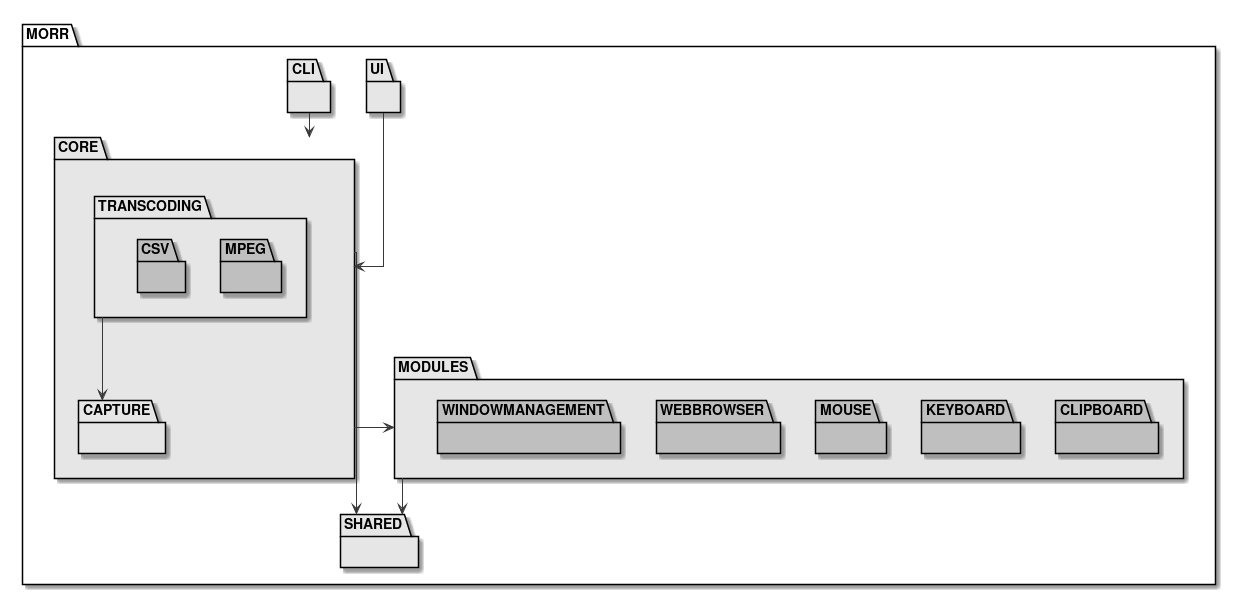
\includegraphics[width=0.80\textwidth]{resources/Packages/AllPackages.png}
\end{center}

The \textbf{MORR} package is the master package containing the whole application. It does not contain any classes directly as it only serves as a container for all packages required in the design.

\begin{packpack}
\packobj{CORE}
\packobj{CLI}
\packobj{SHARED}
\packobj{MODULES}
\packobj{UI}
\end{packpack}

\newpage
\section{MORR.CORE}

\begin{center}
    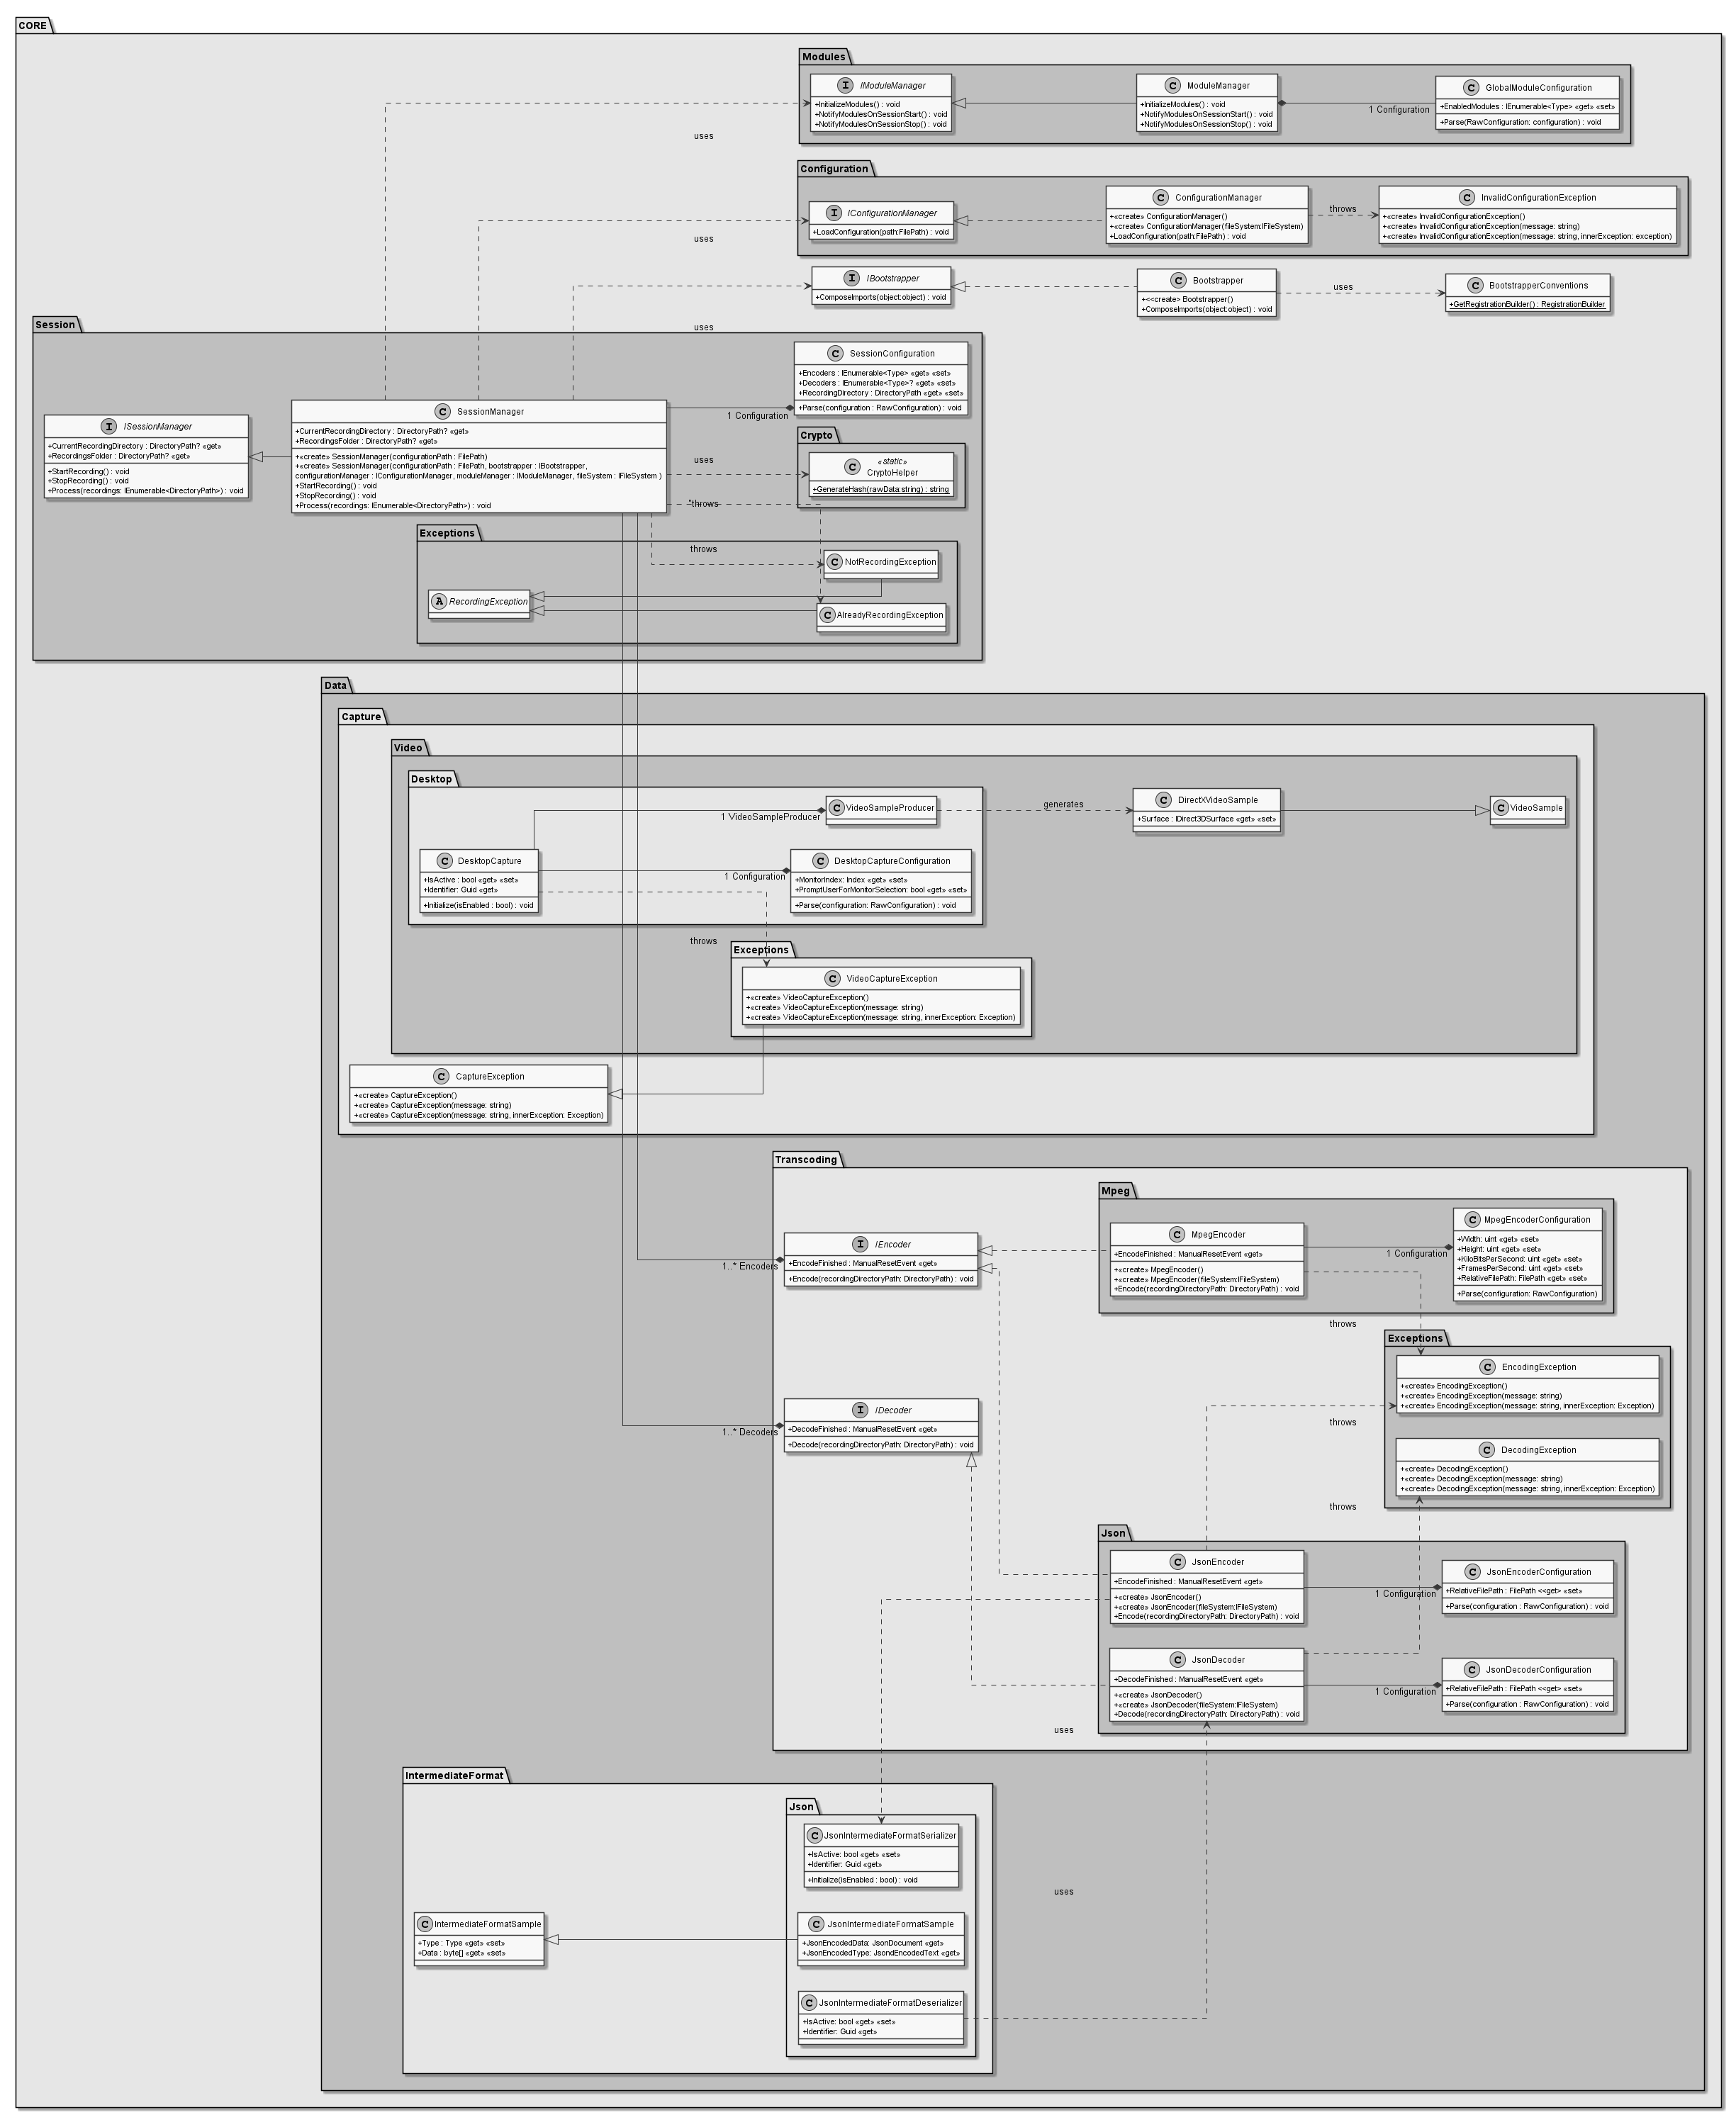
\includegraphics[width=1.0\textwidth]{resources/Packages/CORE.png}
\end{center}

The \textbf{CORE} package contains the compositional facilities required for dynamic composition of the application.

\begin{packif}
\packobj{IBootstrapper}
\end{packif}

\begin{packclass}
\packobj{Bootstrapper}
\packobj{BootstrapperConventions}
\end{packclass}

\begin{packpack}
\packobj{CONFIGURATION}
\packobj{DATA}
\packobj{MODULES}
\packobj{SESSION}
\end{packpack}

\section*{MORR.CORE.CONFIGURATION}

The \textbf{CORE.CONFIGURATION} package is responsible for configuration of the application.

\begin{packif}
\packobj{IConfigurationManager}
\end{packif}

\begin{packclass}
\packobj{ConfigurationManager}
\packobj{InvalidConfigurationException}
\end{packclass}

\section*{MORR.CORE.DATA}

The \textbf{CORE.DATA} package contains all subpackages responsible for data handling.

\begin{packpack}
\packobj{CAPTURE}
\packobj{INTERMEDIATEFORMAT}
\packobj{TRANSCODING}
\end{packpack}

\section*{MORR.CORE.DATA.CAPTURE}

The \textbf{CORE.DATA.CAPTURE} package is responsible for data capture that does not come from modules.

\begin{packclass}
\packobj{CaptureException}
\end{packclass}

\begin{packpack}
\packobj{VIDEO}
\end{packpack}

\section*{MORR.CORE.DATA.CAPTURE.VIDEO}

The \textbf{CORE.DATA.CAPTURE.VIDEO} package is responsible for video capture.

\begin{packclass}
\packobj{DirectXVideoSample}
\packobj{VideoSample}
\end{packclass}

\begin{packpack}
\packobj{DESKTOP}
\packobj{EXCEPTIONS}
\end{packpack}

\section*{MORR.CORE.DATA.CAPTURE.VIDEO.EXCEPTIONS}

\begin{packclass}
\packobj{VideoCaptureException}
\end{packclass}

\section*{MORR.CORE.DATA.CAPTURE.VIDEO.DESKTOP}

The \textbf{CORE.DATA.CAPTURE.VIDEO.DESKTOP} package is responsible for desktop video capture.

\begin{packclass}
\packobj{DesktopCapture}
\packobj{DesktopCaptureConfiguration}
\packobj{VideoSampleProducer}
\end{packclass}

\section*{MORR.CORE.DATA.INTERMEDIATEFORMAT}

The \textbf{CORE.DATA.INTERMEDIATEFORMAT} package is responsible for intermediate format representations.

\begin{packclass}
\packobj{IntermediateFormatSample}
\end{packclass}

\begin{packpack}
\packobj{JSON}
\end{packpack}

\section*{MORR.CORE.DATA.INTERMEDIATEFORMAT.JSON}

The \textbf{CORE.DATA.INTERMEDIATEFORMAT.JSON} package is responsible for JSON intermediate format representations.

\begin{packclass}
\packobj{JsonIntermediateFormatSample}
\packobj{JsonIntermediateFormatSerializer}
\packobj{JsonIntermediateFormatDeserializer}
\end{packclass}

\section*{MORR.CORE.DATA.TRANSCODING}

The \textbf{CORE.DATA.TRANSCODING} package is responsible for transcoding.

\begin{packif}
\packobj{IDecoder}
\packobj{IEncoder}
\end{packif}

\begin{packpack}
    \packobj{EXCEPTIONS}
    \packobj{JSON}
    \packobj{MPEG}
\end{packpack}

\section*{MORR.CORE.DATA.TRANSCODING.EXCEPTIONS}

\begin{packclass}
\packobj{DecodingException}
\packobj{EncodingException}
\end{packclass}

\section*{MORR.CORE.DATA.TRANSCODING.JSON}

The \textbf{CORE.DATA.TRANSCODING.JSON} package is responsible for JSON format transcoding.

\begin{packclass}
    \packobj{JsonDecoder}
    \packobj{JsonDecoderConfiguration}
    \packobj{JsonEncoder}
    \packobj{JsonEncoderConfiguration}
\end{packclass}

\section*{MORR.CORE.DATA.TRANSCODING.MPEG}

The \textbf{CORE.DATA.TRANSCODING.MPEG} package is responsible for MPEG format transcoding.

\begin{packclass}
    \packobj{MpegEncoder}
    \packobj{MpegEncoderConfiguration}
\end{packclass}

\section*{MORR.CORE.MODULES}

The \textbf{CORE.MODULES} package is responsible for module management.

\begin{packif}
\packobj{IModuleManager}
\end{packif}

\begin{packclass}
\packobj{GlobalModuleConfiguration}
\packobj{ModuleManager}
\end{packclass}

\section*{MORR.CORE.SESSION}

The \textbf{CORE.SESSION} package is responsible for session management.

\begin{packif}
\packobj{ISessionManager}
\end{packif}

\begin{packclass}
\packobj{SessionConfiguration}
\packobj{SessionManager}
\end{packclass}

\begin{packpack}
\packobj{EXCEPTIONS}
\packobj{CRYPTO}
\end{packpack}

\section*{MORR.CORE.SESSION.EXCEPTIONS}

\begin{packclass}
\packobj{AlreadyRecordingException}
\packobj{NotRecordingException}
\packobj{RecordingException}
\end{packclass}

\section*{MORR.CORE.SESSION.CRYPTO}

\begin{packclass}
\packobj{CryptoHelper}
\end{packclass}

\newpage
\section{MORR.CLI}

\begin{center}
    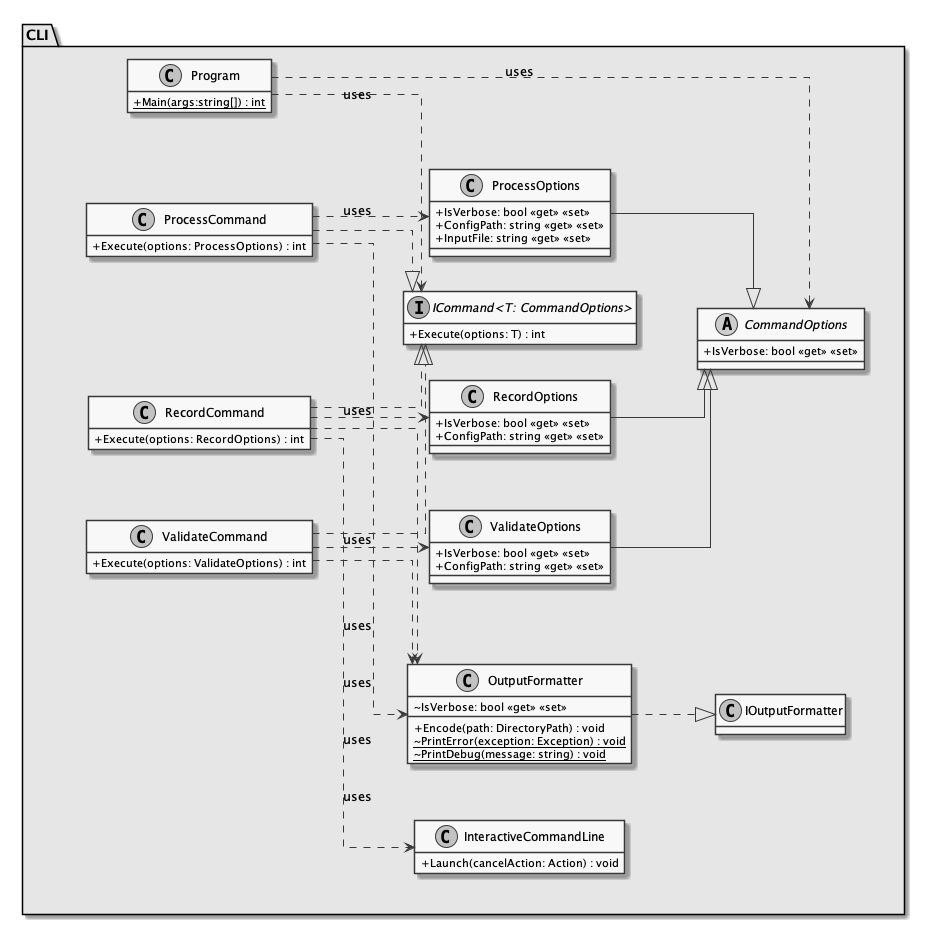
\includegraphics[width=1.0\textwidth]{resources/Packages/CLI.png}
\end{center}

The \textbf{CLI} package contains all logic exclusively needed for the command line interface which allows for the extraction of event data from saved recordings.

\begin{packif}
\packobj{ICommand<T: CommandOptions>}
\packobj{IConsoleFormatter}
\packobj{IMessageLoop}
\packobj{IInteractiveCommandLine}
\end{packif}

\begin{packclass}
\packobj{ConsoleFormatter}
\packobj{CommandOptions}
\packobj{RecordCommand}
\packobj{RecordOptions}
\packobj{ValidateCommand}
\packobj{ValidateOptions}
\packobj{ProcessCommand}
\packobj{ProcessOptions}
\packobj{InteractiveCommandLine}
\packobj{MessageLoop}
\packobj{Program}
\end{packclass}

\newpage
\section{MORR.SHARED}

\begin{center}
    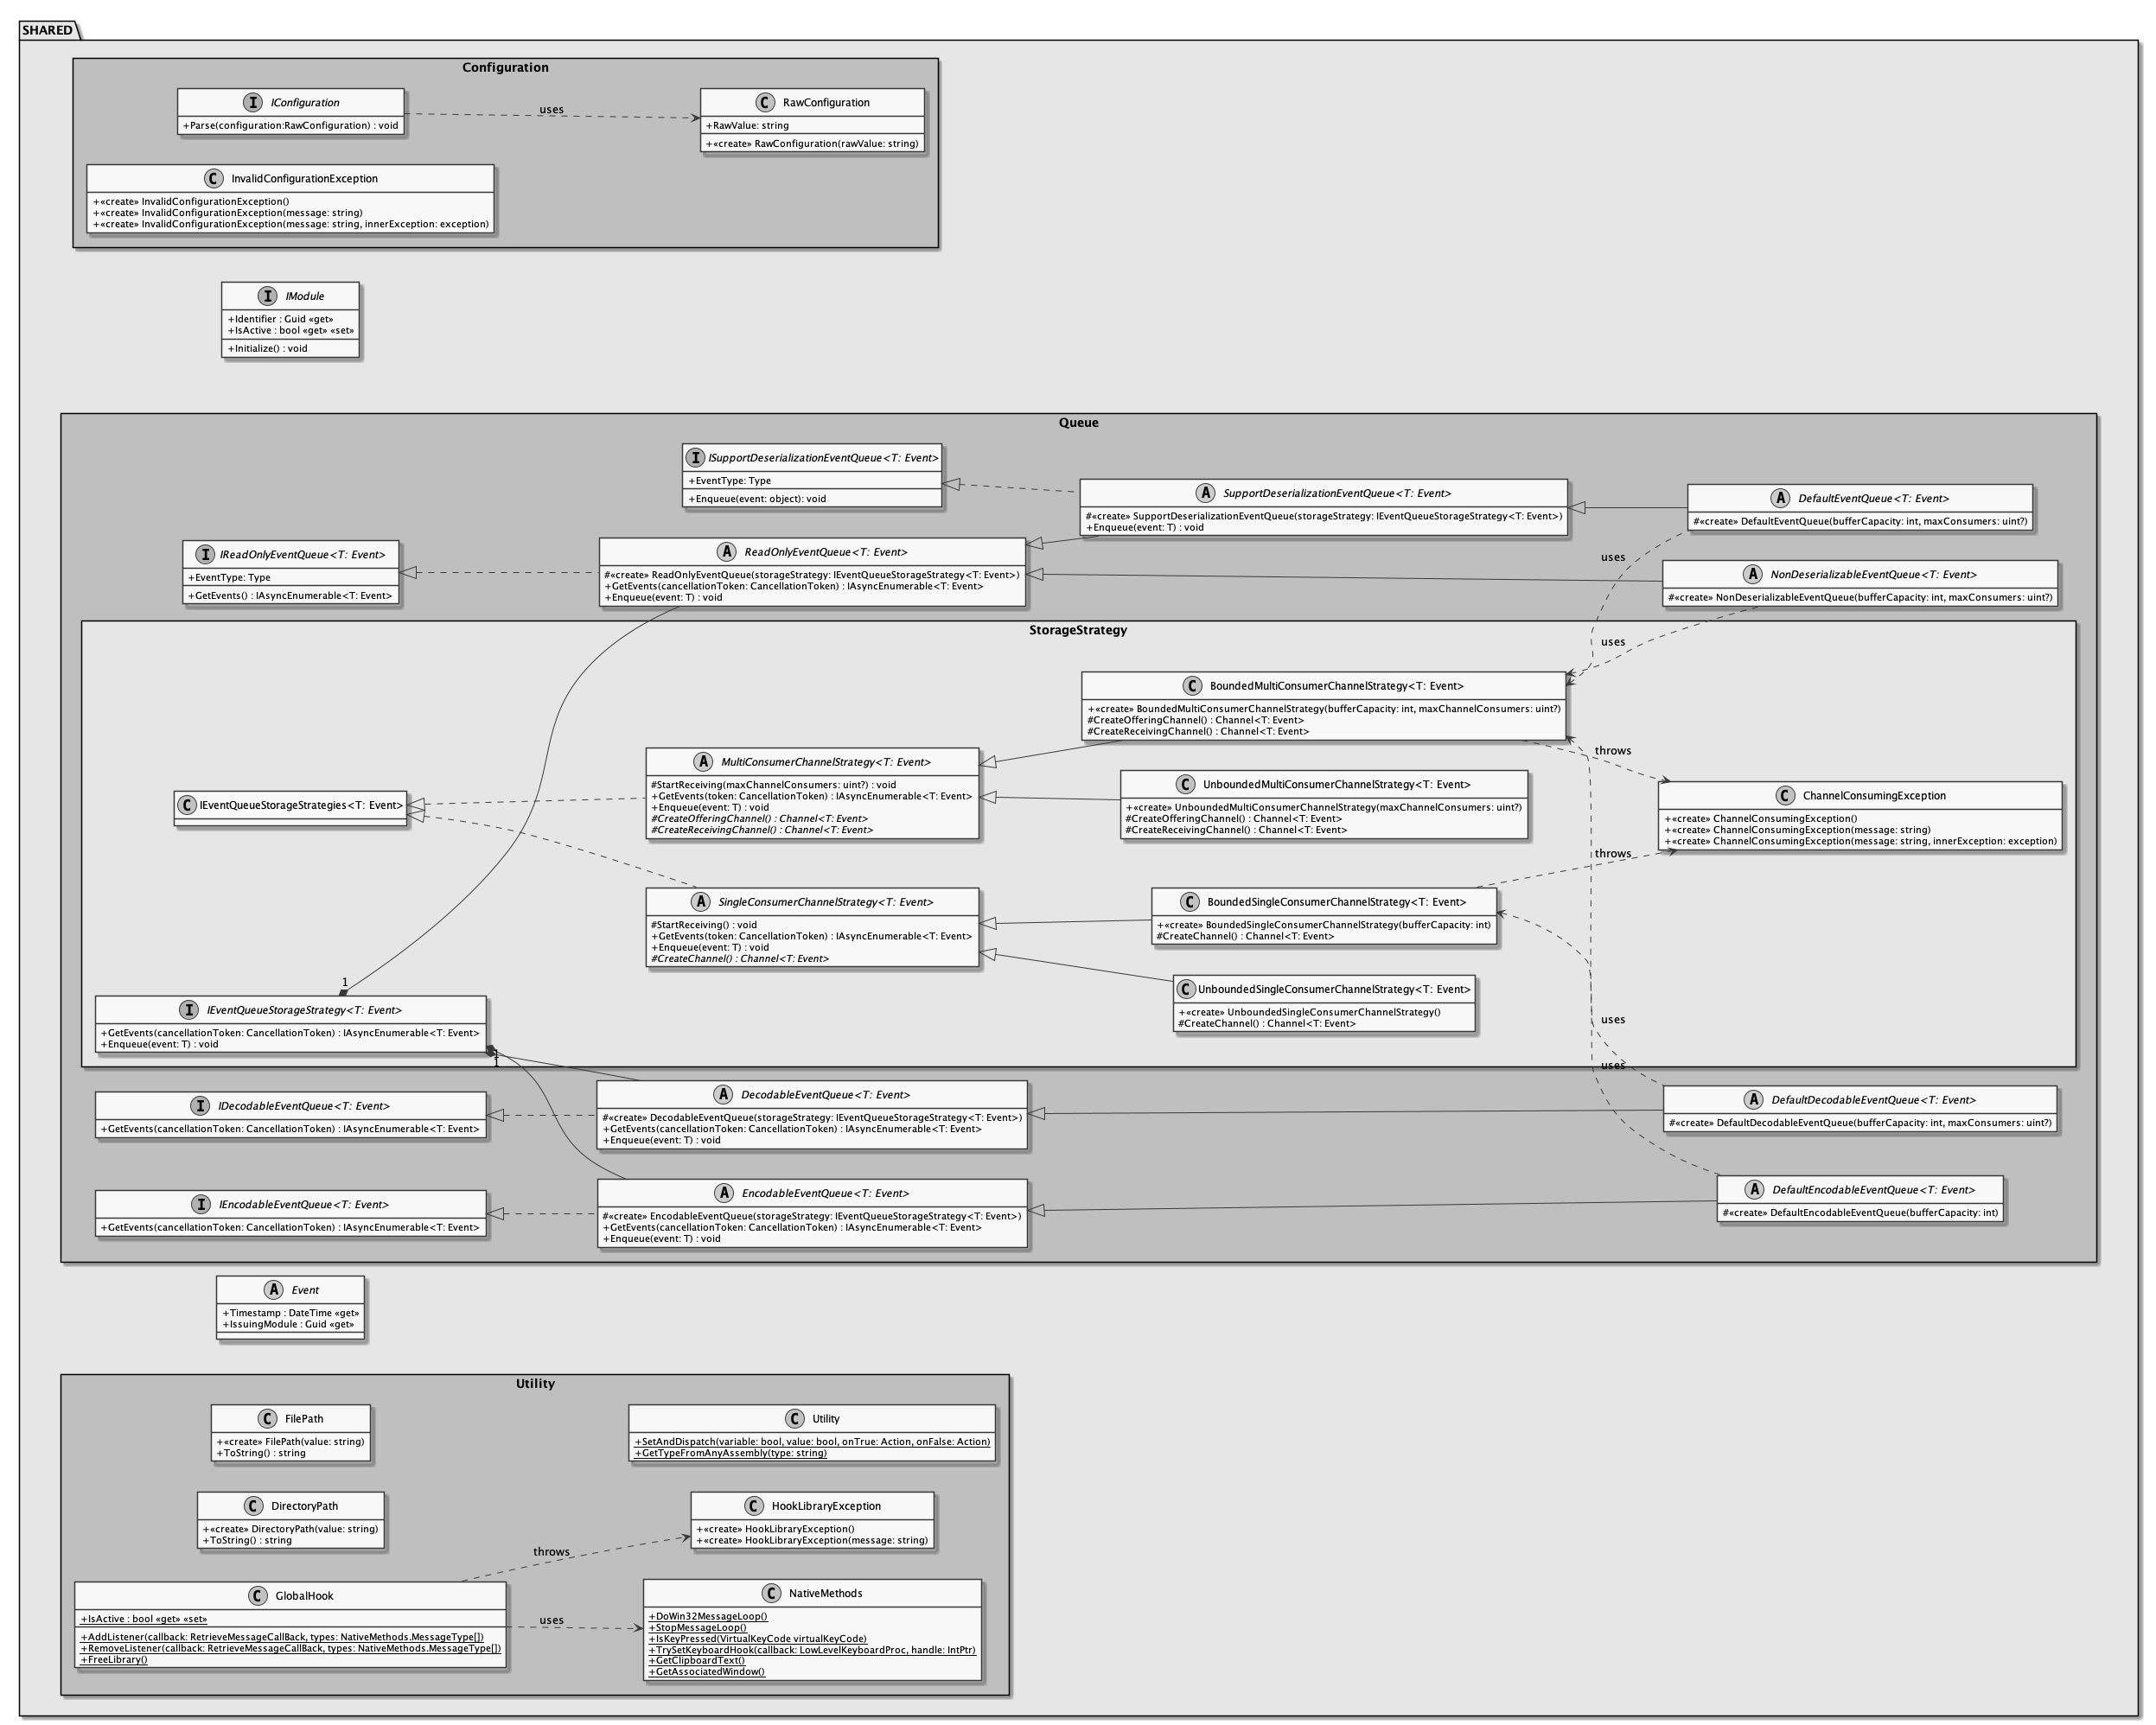
\includegraphics[width=1.0\textwidth]{resources/Packages/SHARED.png}
\end{center}

The \textbf{SHARED} package provides interfaces and classes which have to be known and shared across multiple packages, such as the concept of an event or a module.

\begin{packif}
\packobj{IConfiguration}
\packobj{IModule}
\packobj{IReadOnlyEventQueue<T: Event>}
\packobj{ISupportDeserializationEventQueue<T: Event>}
\packobj{IEventQueueStorageStrategy<T: Event>}
\packobj{IDecodableEventQueue<T: Event>}
\packobj{IEncodableEventQueue<T: Event>}
\end{packif}


\begin{packpack}
\packobj{UTILITY}
\packobj{HOOK}
\packobj{EVENTS}
\packobj{CONFIGURATION}
\packobj{MODULES}
\end{packpack}

\subsection{MORR.SHARED.UTILITY}
\begin{packclass}
\packobj{FilePath}
\packobj{DirectoryPath}
\packobj{Utility}
\end{packclass}

\subsection{MORR.SHARED.CONFIGURATION}
\begin{packclass}
\packobj{RawConfiguration}
\packobj{InvalidConfigurationException}
\end{packclass}

\subsection{MORR.SHARED.HOOK}
\begin{packclass}
\packobj{GlobalHook}
\packobj{HookLibraryException}
\packobj{NativeMethods}
\end{packclass}

\subsection*{MORR.SHARED.EVENTS}
\begin{packclass}
\packobj{\abstract{Event}}
\end{packclass}

\begin{packpack}
\packobj{QUEUE}
\end{packpack}

\subsection*{MORR.SHARED.EVENTS.QUEUE}
\begin{packclass}
\packobj{\abstract{DecodableEventQueue<T: Event>}}
\packobj{\abstract{EncodableEventQueue<T: Event>}}
\packobj{DefaultEncodableEventQueue<T: Event>}
\packobj{DefaultDecodableEventQueue<T: Event>}
\packobj{\abstract{ReadOnlyEventQueue<T: Event>}}
\packobj{\abstract{SupportDeserializationEventQueue<T: Event>}}
\packobj{DefaultEventQueue<T: Event>}
\packobj{NonDeserializableEventQueue<T: Event>}
\end{packclass}

\begin{packpack}
\packobj{STORAGESTRATEGY}
\end{packpack}

\subsubsection*{MORR.SHARED.EVENTS.QUEUE.STORAGESTRATEGY}
\begin{packclass}
\packobj{\abstract{MultiConsumerChannelStrategy<T: Event>}}
\packobj{\abstract{SingleConsumerChannelStrategy<T: Event>}}
\packobj{BoundedMultiConsumerChannelStrategy<T: Event>}
\packobj{UnboundedMultiConsumerChannelStrategy<T: Event>}
\packobj{BoundedSingleConsumerChannelStrategy<T: Event>}
\packobj{UnboundedSingleConsumerChannelStrategy<T: Event>}
\packobj{ChannelConsumingException}
\end{packclass}


\newpage
\section{MORR.MODULES}

The \textbf{MODULES} package serves as a container for all module-subpackages.

\begin{packpack}
\packobj{WINDOWMANAGEMENT}
\packobj{KEYBOARD}
\packobj{CLIPBOARD}
\packobj{WEBBROWSER}
\packobj{MOUSE}
\end{packpack}

\subsection*{MORR.MODULES.WINDOWMANAGEMENT}

\begin{center}
    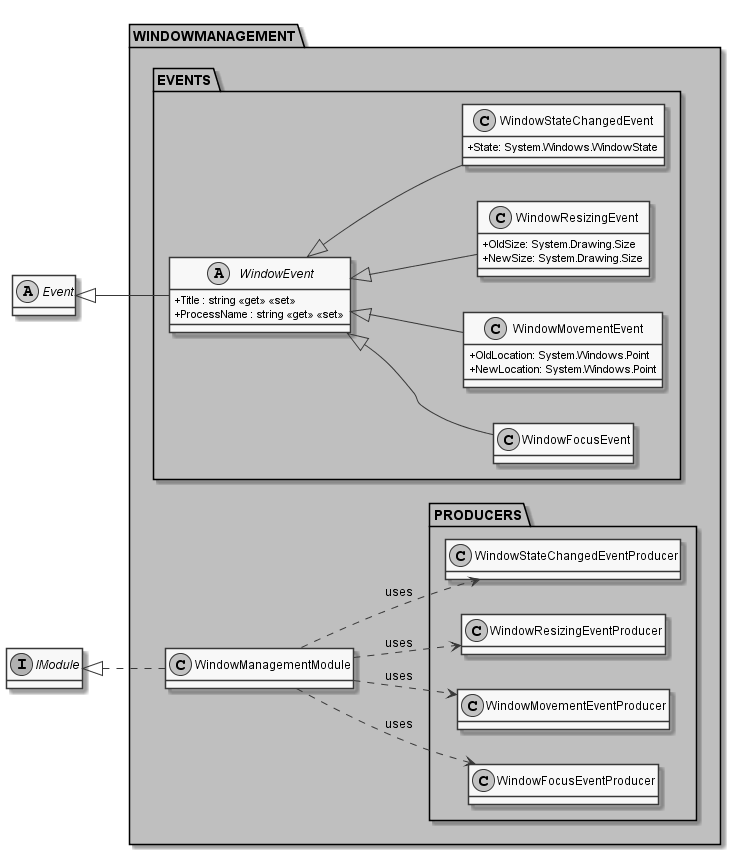
\includegraphics[width=1.0\textwidth]{resources/Packages/MODULES_WINDOWMANAGEMENT.png}
\end{center}

The \textbf{MODULES.WINDOWMANAGEMENT} package is responsible for providing the classes and concepts necessary for recording the window related user-interactions.

\begin{packclass}
\packobj{WindowManagementModule}
\end{packclass}

\begin{packpack}
\packobj{EVENTS}
\packobj{PRODUCERS}
\end{packpack}

\subsection*{MORR.MODULES.WINDOWMANAGEMENT.EVENTS}
\begin{packclass}
\packobj{\abstract{WindowEvent}}
\packobj{WindowMovementEvent}
\packobj{WindowFocusEvent}
\packobj{WindowSateChangedEvent}
\packobj{WindowResizingEvent}
\end{packclass}

\subsection*{MORR.MODULES.WINDOWMANAGEMENT.PRODUCERS}
\begin{packclass}
\packobj{WindowMovementEventProducer}
\packobj{WindowFocusEventproducer}
\packobj{WindowSateChangedEventProducer}
\packobj{WindowResizingEventProducer}
\end{packclass}
\newpage

\subsection*{MORR.MODULES.KEYBOARD}

\begin{center}
    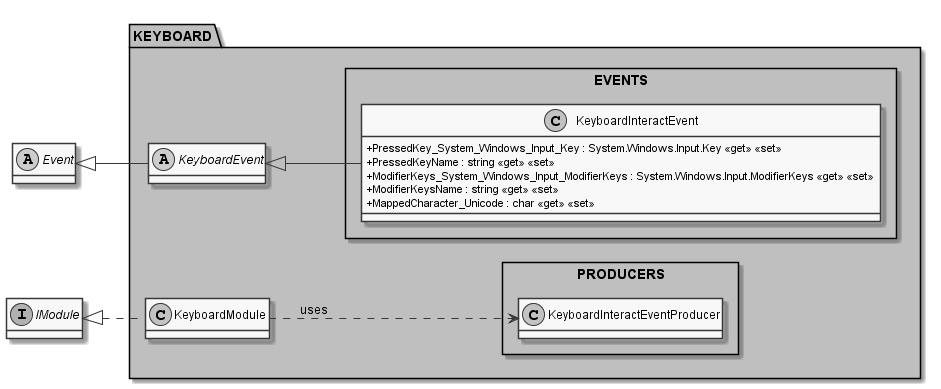
\includegraphics[width=1.0\textwidth]{resources/Packages/MODULES_KEYBOARD.png}
\end{center}

The \textbf{MODULES.KEYBOARD} package is responsible for providing the classes and concepts necessary for recording the keyboard related user-inputs.

\begin{packclass}
\packobj{KeyboardModule}
\end{packclass}

\begin{packpack}
\packobj{EVENTS}
\packobj{PRODUCERS}
\end{packpack}

\subsection*{MORR.MODULES.KEYBOARD.EVENTS}
\begin{packclass}
\packobj{\abstract{KeyboardEvent}}
\packobj{KeyboardInteractEvent}
\end{packclass}

\subsection*{MORR.MODULES.KEYBOARD.PRODUCERS}
\begin{packclass}
\packobj{KeyboardInteractEventProducer}
\end{packclass}

\newpage
\subsection*{MORR.MODULES.WEBBROWSER}

\begin{center}
    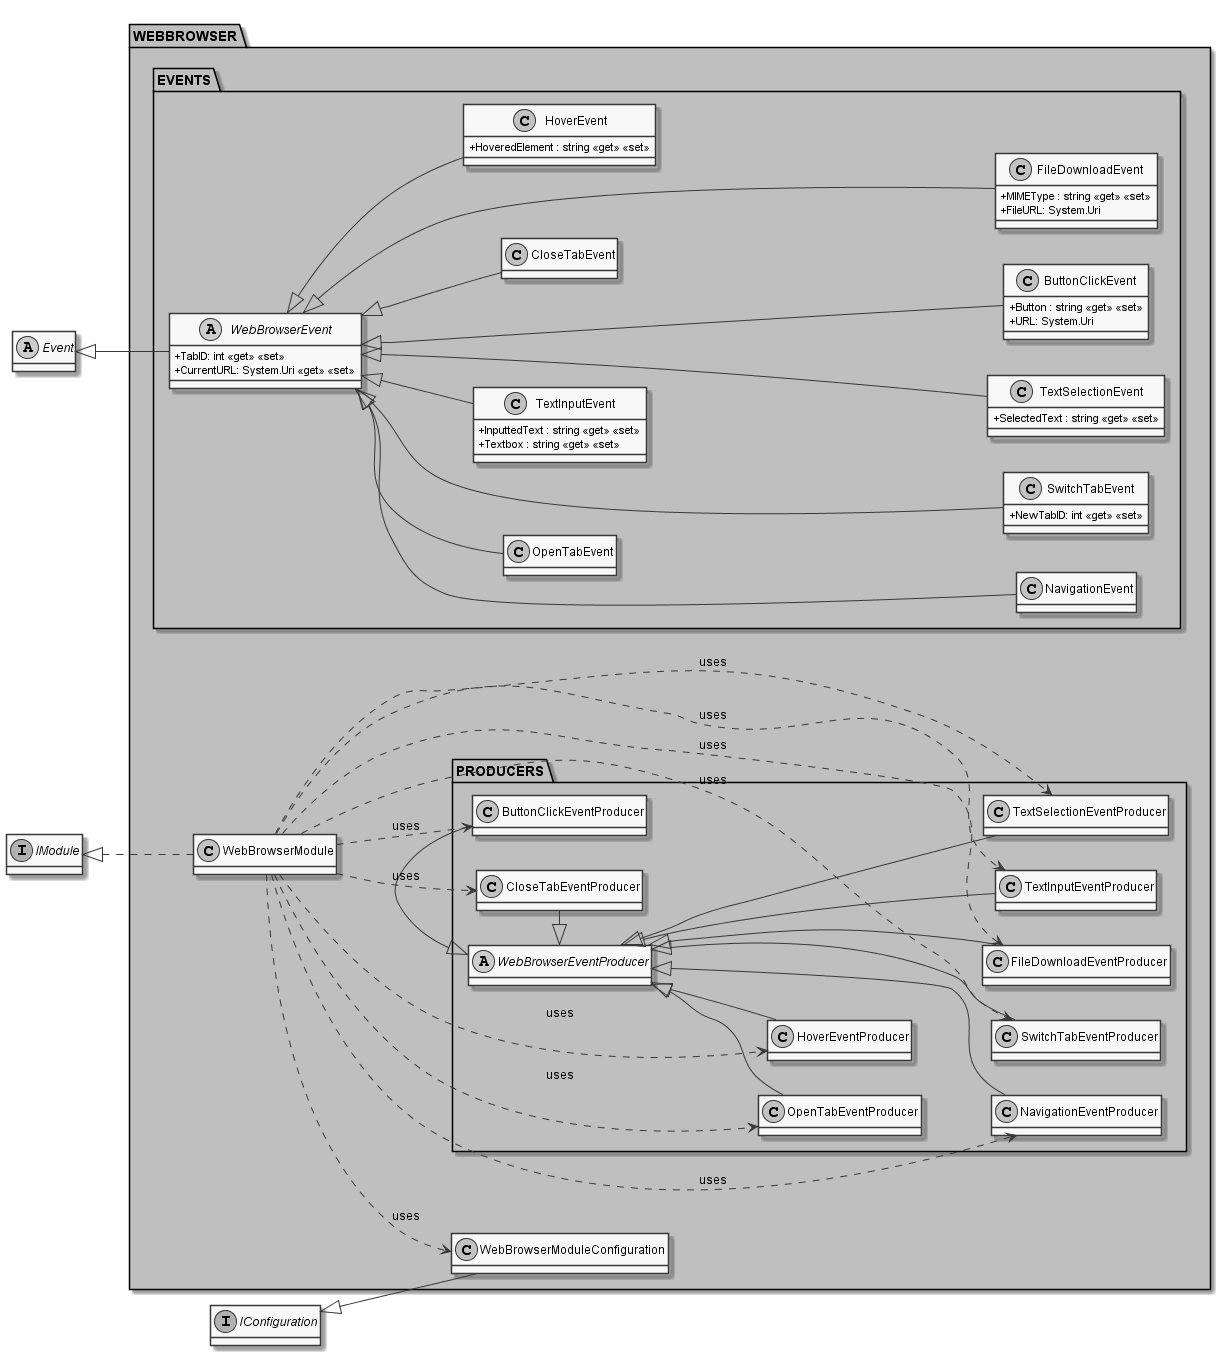
\includegraphics[width=1.0\textwidth]{resources/Packages/MODULES_WEBBROWSER.png}
\end{center}

The \textbf{MODULES.WEBBROWSER} package is responsible for providing the classes and concepts necessary for recording the webbrowser related user-interactions.

\begin{packclass}
\packobj{WebBrowserModule}
\packobj{WebBrowserModuleConfiguration}
\end{packclass}

\begin{packpack}
\packobj{EVENTS}
\packobj{PRODUCERS}
\end{packpack}

\subsection*{MORR.MODULES.WEBBROWSER.EVENTS}
\begin{packclass}
\packobj{\abstract{WebBrowserEvent}}
\packobj{TextSelectionEvent}
\packobj{TextInputEvent}
\packobj{SwitchTabEvent}
\packobj{OpenTabEvent}
\packobj{CloseTabEvent}
\packobj{NavigationEvent}
\packobj{HoverEvent}
\packobj{FileDownloadEvent}
\packobj{ButtonClickEvent}

\end{packclass}

\subsection*{MORR.MODULES.WEBBROWSER.PRODUCERS}
\begin{packclass}
\packobj{\abstract{WebBrowserEventProducer}}
\packobj{TextSelectionEventProducer}
\packobj{TextInputEventProducer}
\packobj{SwitchTabEventProducer}
\packobj{OpenTabEventProducer}
\packobj{CloseTabEventProducer}
\packobj{NavigationEventProducer}
\packobj{HoverEventProducer}
\packobj{FileDownloadEventProducer}
\packobj{ButtonClickEventProducer}
\end{packclass}


\newpage
\subsection*{MORR.MODULES.CLIPBOARD}

\begin{center}
    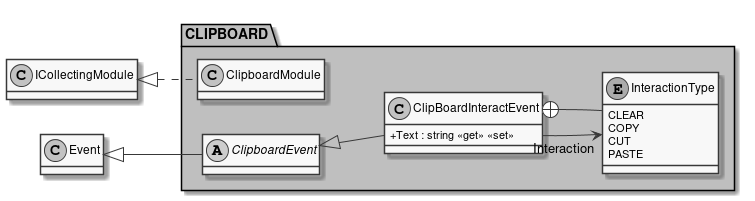
\includegraphics[width=1.0\textwidth]{resources/Packages/MODULES_CLIPBOARD.png}
\end{center}

The \textbf{MODULES.CLIPBOARD} package is responsible for providing the classes and concepts necessary for recording the clipboard related user-interactions.

\begin{packclass}
\packobj{ClipboardModule}
\end{packclass}

\begin{packpack}
\packobj{EVENTS}
\packobj{PRODUCERS}
\end{packpack}

\subsection*{MORR.MODULES.CLIPBOARD.EVENTS}
\begin{packclass}
\packobj{\abstract{ClipboardEvent}}
\packobj{ClipboardCopyEvent}
\packobj{ClipboardCutEvent}
\packobj{ClipboardPasteEvent}
\end{packclass}

\subsection*{MORR.MODULES.CLIPBOARD.PRODUCERS}
\begin{packclass}
\packobj{ClipboardCopyEventProducer}
\packobj{ClipboardCutEventProducer}
\packobj{ClipboardPasteEventProducer}
\end{packclass}



\newpage
\subsection*{MORR.MODULES.MOUSE}

\begin{center}
    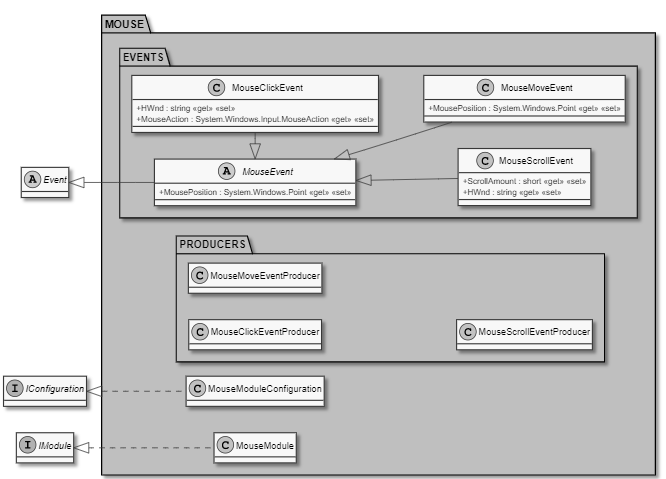
\includegraphics[width=1.0\textwidth]{resources/Packages/MODULES_MOUSE.png}
\end{center}

The \textbf{MODULES.MOUSE} package is responsible for providing the classes and concepts necessary for recording the mouse related user-inputs.

\begin{packclass}
\packobj{MouseModule}
\packobj{MouseModuleConfiguration}
\end{packclass}

\begin{packpack}
\packobj{EVENTS}
\packobj{PRODUCERS}
\end{packpack}

\subsection*{MORR.MODULES.MOUSE.EVENTS}
\begin{packclass}
\packobj{\abstract{MouseEvent}}
\packobj{MouseScrollEvent}
\packobj{MouseClickEvent}
\packobj{MouseMoveEvent}
\end{packclass}

\subsection*{MORR.MODULES.MOUSE.PRODUCERS}
\begin{packclass}
\packobj{MouseScrollEventProducer}
\packobj{MouseClickEventProducer}
\packobj{MouseMoveEventProducer}
\end{packclass}

\newpage

\section{MORR.UI}

\begin{center}
    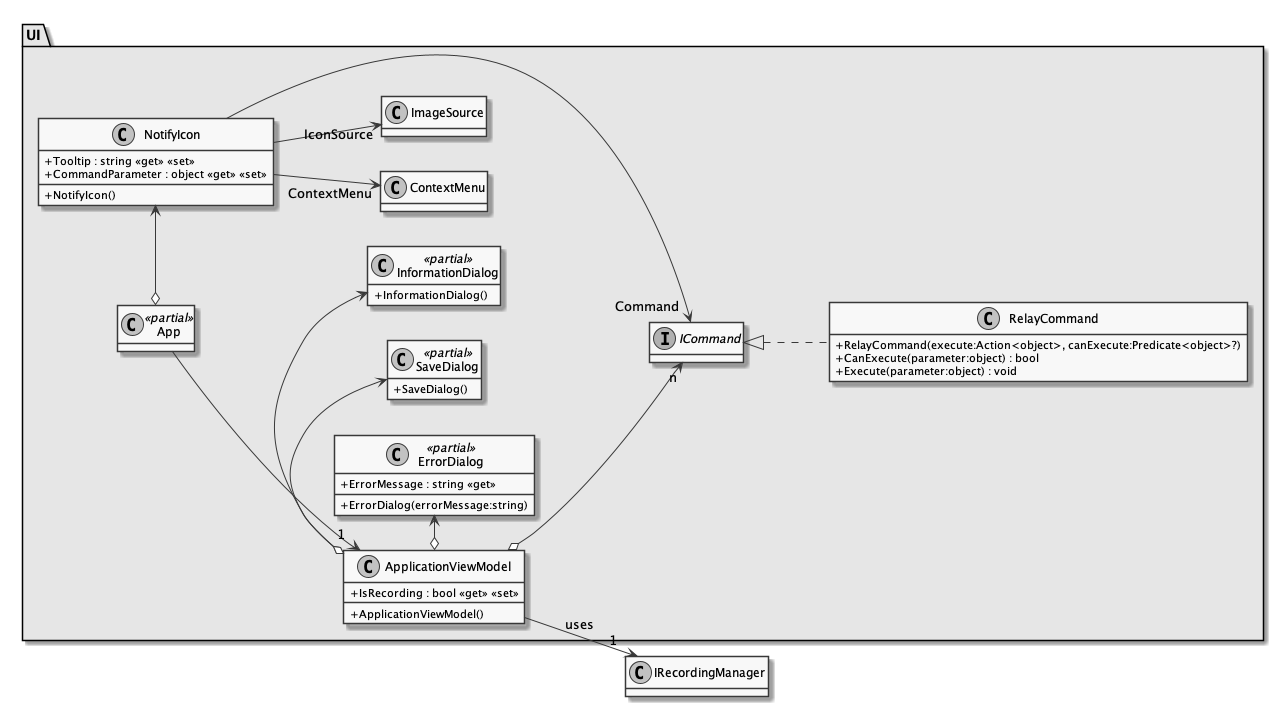
\includegraphics[width=1.0\textwidth]{resources/Packages/UI.png}
\end{center}

The \textbf{UI} package is responsible for the graphical user interface.

\begin{packclass}
\packobj{NotifyIcon}
\packobj{<<partial> App}
\packobj{<<partial>> InformationDialog}
\packobj{<<partial>> ConfirmationDialog}
\packobj{<<partial>> SaveDialog}
\packobj{<<partial>> ErrorDialog}
\packobj{ApplicationViewModel}
\packobj{RelayCommand}
\end{packclass}
